%%%%%%%%%%%%%%%%%%%%%%%%%%%%%%%%%%%%%%%%%%%%%%%%%
%------ LaTeX-Template
%%%%%%%%%%%%%%%%%%%%%%%%%%%%%%%%%%%%%%%%%%%%%%%%%

%---- Header (mit Formateinstellugen) laden, Inputencoding prüfen ------

%%%%%%%%%%%%%%%%%%%%%%%%%%%%%%%%%%%%%%%%%%%%%%%%%
%---- LaTeX-Header
%%%%%%%%%%%%%%%%%%%%%%%%%%%%%%%%%%%%%%%%%%%%%%%%%

\documentclass[12pt,paper=A4,numbers=noenddot,bibliography=totoc,listof=totoc,DIV=11,BCOR=1mm]{scrreprt}
%  Bindekorrektur BCOR (verlorener Rand am linken Blattrand)! Wert haengt von der Art der Heftung ab!!
%  Satzspiegeleinstellung DIV von KOMA-Script / sccreprt.

\pagestyle{headings}

\usepackage[T1]{fontenc} % Font Encoding fuer europaeische Schriften mit Umlauten (Unterstuetzung der Worttrennung)
\usepackage{lmodern} % PostScript-Varianten der TeX Computer Modern-Schriften laden
\usepackage[english,ngerman]{babel} % Spracheinstellungen fuer Englisch und Neudeutsch laden

\usepackage{setspace}

\usepackage{graphicx} % Grafikeinbindung (fuer .JPG, .JPEG, .PNG und .PDF, falls pdflatex benutzt wird)
\usepackage[table]{xcolor} % ermoeglicht farbige Schrift und farbige Tabellenzeilen
\definecolor{black}{gray}{0} % Umdefinition der Farbe black, falls noetig (0=schwarz, 1=weiss)
\definecolor{dblue}{rgb}{0.1,0.2,0.6} % Dunkelblau, fuer Hyperlinks
\definecolor{lgray}{gray}{0.9} % Hellgrau, fuer Tabellen (0=schwarz, 1=weiss)

\usepackage{booktabs} % fuer schoene Tabellen

\usepackage[round,authoryear]{natbib} % Literaturverweise mit Name/Jahreszahl in runden Klammern
\bibpunct[:\,]{(}{)}{,}{a}{}{,~}  % Feinformatierung der Natbib-Zitierweise

\usepackage[hyphens]{url}
\usepackage[colorlinks=true,linkcolor=black,citecolor=dblue,urlcolor=dblue]{hyperref} 
\usepackage{hyperref}  
% die Pakete url und hyperref ermoeglichen anklickbare URLs im Quellenverzeichnis in definierter Farbe, 
% sie ermoeglichen den Zeilenumbruch bei langen URLs, und sie erzeugen Hyperlinks (Farbe s.o.) 
% zwischen Quellenverweis und Quellenverzeichnis sowie zwischen label und ref im PDF-Dokument

\usepackage[section]{placeins}
% Fonteinstellungen fuer Bildunterschriften: Unterschrift serifenlos, "Abbildung" fett (bfseries = bold face series)
\setkomafont{captionlabel}{\sffamily\bfseries}
\setkomafont{caption}{\sffamily}

%------------------------------------------------------------------------------------------------------------------
%------ Eigenstaendigkeitserklaerung im gerahmten Kasten (parbox in einer framebox) ------
%------------------------------------------------------------------------------------------------------------------

\newcommand{\eigen}{
\setlength{\fboxsep}{2ex}
\setlength{\fboxrule}{0.8pt} 
% Einstellungen fuer Rahmenabstand und Rahmendicke der Framebox
\begin{center}
	\fbox{
		\parbox{0.8\linewidth}{
		Ich versichere, die vorliegende Arbeit selbstst\"andig ohne fremde Hilfe verfasst 
		und keine anderen Quellen und Hilfsmittel als die angegebenen benutzt zu haben. 
		Die aus anderen Werken w\"ortlich entnommenen Stellen oder dem Sinn nach 
		entlehnten Passagen sind durch Quellenangaben eindeutig kenntlich gemacht.
		\par\bigskip\bigskip\bigskip\bigskip
		\hspace*{0.8cm}Ort, Datum \hfill \vorname~\nachname\hspace*{0.8cm}
		}
	}
\end{center}
}

%%%%%%%%%%%%%%%%%%%%%%%%%%%%%%%%%%%%%%%%%%%%%%%%%

%\usepackage[applemac]{inputenc} % Inputencoding f�r Mac
%\usepackage[latin1]{inputenc} % Inputencoding f�r PC/Win
\usepackage[utf8]{inputenc} % Inputencoding, universell
%\usepackage[utf8x]{inputenc} % Inputencoding, universell


%------------------------ Titelblatt-Layout laden ----------------------------------

%%%%%%%%%%%%%%%%%%%%%%%%%%%%%%%%%%%%%%%%%%%%%%%%%
%------ LaTeX-Titelblatt
%------ Deklarationen fuer die Titelseite
%%%%%%%%%%%%%%%%%%%%%%%%%%%%%%%%%%%%%%%%%%%%%%%%%

\title{\titel\\[2ex]
\LARGE Bachelor-Thesis\\
\large zur Erlangung des akademischen Grades B.Sc.\\[1.5ex]
\LARGE \vorname~\nachname\\[0.5ex] 
\large \matrikelnummer
}

\author{\unitlength1mm
\large\raisebox{-1ex}{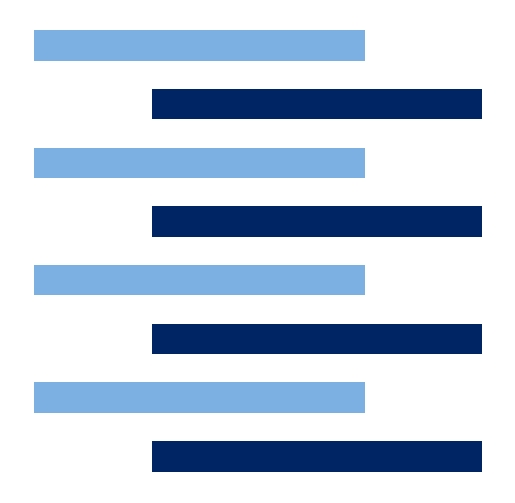
\includegraphics[width=4em]{HAW_wuerfel}}\hspace{1ex}
\parbox[b]{11.2cm}{\sffamily\large%
Hochschule für Angewandte Wissenschaften Hamburg\\[-0.2ex]
Fakultät Design, Medien und Information\\[-0.2ex]
Department Medientechnik
}\\[6ex]
\sffamily\large Erstprüfer: \erstpruef\\[0.5ex]
\sffamily\large Zweitprüfer: \zweitpruef}

%%%%%%%%%%%%%%%%%%%%%%%%%%%%%%%%%%%%%%%%%%%%%%%%%

%---------------------------- Titeldefinitionen --------------------------------------

\newcommand{\vorname}{Sebastian}
\newcommand{\nachname}{Bohn}
\newcommand{\matrikelnummer}{2036605}

\newcommand{\titel}{Analyse und Evaluierung von plattformübergreifenden Spiel-Engines und Frameworks,anhand der Implementierung einer mobilen Beispielapplikation}

\newcommand{\erstpruef}{Prof. Dr. Edmund Weitz}
\newcommand{\zweitpruef}{Prof. Dr. Andreas Plaß}

\date{vorläufige Fassung vom \today}   % Vorab-Version 
%\date{\sffamily Hamburg, DD. MM. YYYY}  % Abgabedatum!

%----------------------------- ANFANG --------------------------------------

\begin{document}
\selectlanguage{ngerman}
\setlength{\parindent}{0em}
% Titelseite erzeugen
\maketitle
% Inhaltsverzeichnis erzeugen          
\tableofcontents
% Seitenumbruch
\clearpage

%----------------------------INHALT---------------------------------------

%---------------------------ABSTRACT------------------------------------

\thispagestyle{empty}
\selectlanguage{english}
\section*{\centering\abstractname}

%TODO: English abstract

\selectlanguage{ngerman}
\section*{\centering\abstractname}

%TODO: Deutsches abstract

%----------------------------TEXT-----------------------------------------------

%TODO: Kapitel 1
\chapter{Einleitung}

\section{Motivation}
\section{Gliederung}

%TODO: Kapitel 2
\chapter{Mobile Systeme}

\section{Aktuelle Systeme auf dem mobilen Markt}

\subsection{iOS}
iOS ist das mobile Betriebssystem des Unternehmen Apple. Dieses ist ein Derivat von Mac OS X, welches selbst auf Unix basiert. Es wird ausschließlich von Apple entwickelt und ist somit nur auf den eigenen Geräten iPhone, iPad und iPod touch zu finden. Mit der Entwicklung wurde unter externer und interner Geheimhaltung 2005 begonnen und das Resultat der Öffentlichkeit zum ersten Mal Anfang 2007 vorgestellt. Bis zur Version 4.0 wurde iOS mit dem Namen iPhoneOS betitelt. Das Konzept und Design ist schwerpunktmäßig auf hohe Benutzerfreundlichkeit und Funktionalität ausgelegt. 

Durch die geschlossene Struktur des Systems sind eigene Derivate nicht möglich. Entwickler haben die Möglichkeit, durch das iOS Software Development Kit (SDK) eigene Applikationen zu entwickeln und in Apples App Store zu veröffentlichen.
Bei der Wahl der Hardware ist man auf die Produktpalette von Apple angewiesen, welche jährlich eine neue Generation veröffentlicht. Die Personalisierung der Geräte ist nur bedingt möglich, da Anbieter von Drittsoftware keinen Zugriff auf das System haben und Anwendungen nur offiziell über den eigenen App Store bezogen werde können. Dies bietet jedoch den Vorteil einer Qualitätssicherung durch Apple, da Applikationen vor der Veröffentlichung einer Prüfung unterzogen werden.
\\

\textbf{Vorteile:}
\begin{itemize}
	\item Kompatibilität von Software und Hardware
	\item Benutzerfreundlichkeit
	\item Geräteübergreifende Kommunikation
	\item Kontrollen bei Veröffentlichung von Anwendungen
\end{itemize}

\textbf{Nachteile:}
\begin{itemize}
	\item Restriktive Firmenpolitik
	\item Proprietäres System
	\item Hardwareauswahl
	\item Anwendungen nur über den App Store
\end{itemize}

\subsection{Android}
Android ist ein Open Source Betriebssystem und gleichzeitig eine Software-Plattform, welches stark im mobilen Bereich vertreten ist und auf dem Linux-Kernel basiert. Zu finden ist diese auf Smartphones, Tablet-Computern, Netbooks und auch auf Smart-TV Geräten.\citep{android_overview} Entwickelt wird Android von der Open Handset Alliance (OHA), welche von Google gegründet wurde. Die OHA wurde im November 2007 gegründet und ist ein Konsortium von mehr als 80 Unternehmen aus den Bereichen Mobilfunknetz, Geräteherstellung, Halbleiterindustrie, Marketing und Software. \citep{alliance_members} Der Grund für die Entwicklung von Android war und ist es, einen offenen Standard für mobile Geräte zu schaffen.\cite{alliance_overview}

Durch seine Offenheit ermöglicht Android Entwicklern große Freiheit bei der Programmierung von Applikationen. Eigene Entwicklungen können auch mit Anwendungen von Google, wie zum Beispiel Google Maps, verknüpft werden.
Auch der Hardwarebereich bietet ein breites Spektrum an Geräten mit kostengünstigen, bis hochpreisigen Angeboten, sowohl mit einfacher bis qualitativ hochwertiger, technischer Ausstattung. Benutzer haben die Möglichkeit, ihre Geräte weitestgehend frei zu gestalten und einzustellen. Bei der Installation von Anwendungen sind sie auch nicht zwangsläufig an einen Anbieter gebunden.
\\

Vorteile:
\begin{itemize}
	\item Open Source
	\item Unabhängigkeit von Anbietern
	\item Personalisierung
	\item Hardwareangebot
\end{itemize}

Nachteile:
\begin{itemize}
	\item Hohe Verbreitung von Schadsoftware
	\item Aktualität der Version ist abhängig vom Gerätehersteller
\end{itemize}

\subsection{Windows Phone}
\subsection{Weitere Systeme}

\section{Bedarfsanalyse}
\subsection{Markt- und Useranteile der jeweiligen Systeme}
\subsection{Verfügbare Applikationen / Games der Stores}

%TODO: Kapitel 3
\chapter{Native Softwareentwicklung}
Softwareentwicklung für ein bestimmtes System wird als nativ (lat.: angeboren, natürlich) bezeichnet. Hier sind Dateiformate, Programmiersprachen, Hardware, Entwicklungsumgebungen und Kompilierung genau an die Zielplattform angepasst. Nativer Code ist in der Lage alle individuellen Eigenschaften einer Zielplattform anzusprechen, ohne dabei eine eventuelle Portierbarkeit zu berücksichtigen.
\citep{native_software}
Welche Anforderungen iOS, Android und Windows Phone bezüglich nativer Entwicklung voraussetzen, soll in diesem Kapitel näher erläutert werden.

\section{Systemvorraussetzungen}
Um eine Applikation für eine bestimmte Zielplattform zu entwickeln, ist es unter Umständen nötig die Voraussetzung eines bestimmten Betriebssystems zu erfüllen.

\subsection{iOS}
%TODO

\subsection{Android}
Die Entwicklung von Android Applikationen ist an kein bestimmtes System gebunden und somit lassen sich diese unter Windows, OS X und Linux Systemen. 
Windows Benutzer sollten mindestens Windows XP nutzen. Darüber hinaus können alle aktuelleren Versionen genutzt werden, wobei alle 32-Bit Editionen unterstützt werden und ab Windows 7 auch die mit 64-Bit.
Mac Systeme werden ab OS X 10.5.8 von den offiziellen Entwicklungswerkzeugen unterstützt.
Um auf einem Linux System zu entwickeln, kann man dies beispielsweise unter Ubuntu ab Version 8.04 tun. Bei 64-Bit Versionen ist es notwendig, dass diese fähig ist 32-Bit Anwendungen auszuführen. Da die Auswahl an Linux-Distributionen sehr umfangreich ist, wird an dieser Stelle auf diese nicht weiter eingegangen.
\citep{android_sdk_requirements}

\subsection{Windows Phone}
%TODO

\section{SDKs und Versionen}
Software Development Kits, kurz SDKs, liefern dem Entwickler die Werkzeuge, Anwendungen und bestenfalls eine aktuelle Dokumentation, um für eine bestimmte Zielplattform zu entwickeln. Auch sind sie notwendig, um geschriebenen Code zu interpretieren und kompilieren. Um die aktuellste Version eines mobilen Systems zu unterstützen, muss das SDK auf ebenso aktuellen Stand sein.

\subsection{iOS Versionen}
Apple nutzt für seine Produkte Codenamen, die keinem bestimmten Muster folgen. Verbrauchern sind diese meist unbekannt, da diese überwiegend intern genutzt werden.
\begin{table}[htbp]
\centering
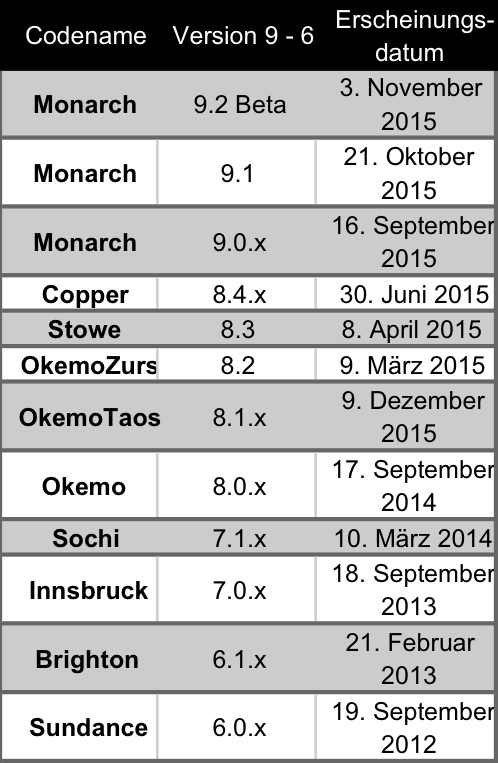
\includegraphics[width=0.5\textwidth]{Tabellen/iOS_Versionen_9-6}
\caption{iOS Versionen 9 - 6 und ihr Erscheinungsdatum}\label{tab_ios_vers_9-6}\citep{ios_codenames}
\end{table}
\begin{table}[htbp]
\centering
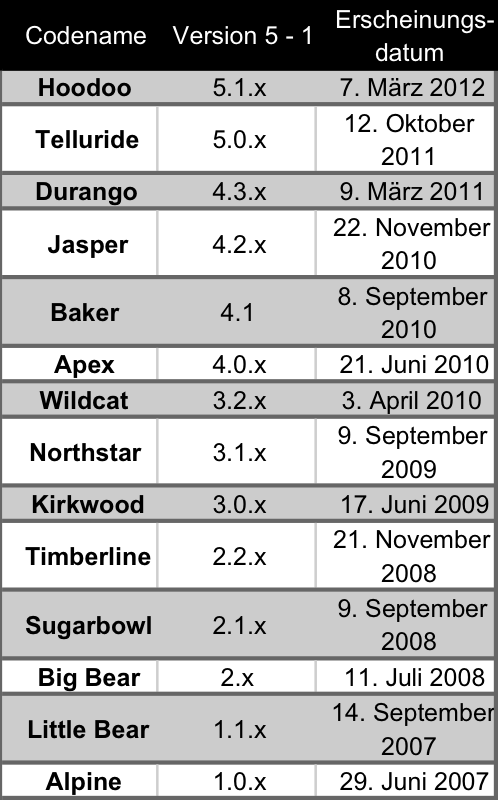
\includegraphics[width=0.5\textwidth]{Tabellen/iOS_Versionen_5-1}
\caption{iOS Versionen 5 - 1 und ihr Erscheinungsdatum}\label{tab_ios_vers_5-1}\citep{ios_codenames}
\end{table}
\clearpage

\subsection{Android Versionen}
Android Versionen sind nach süßen Leckereien benannt und dem Anfangsbuchstaben nach alphabetisch aufsteigend.
\begin{table}[htbp]
\centering
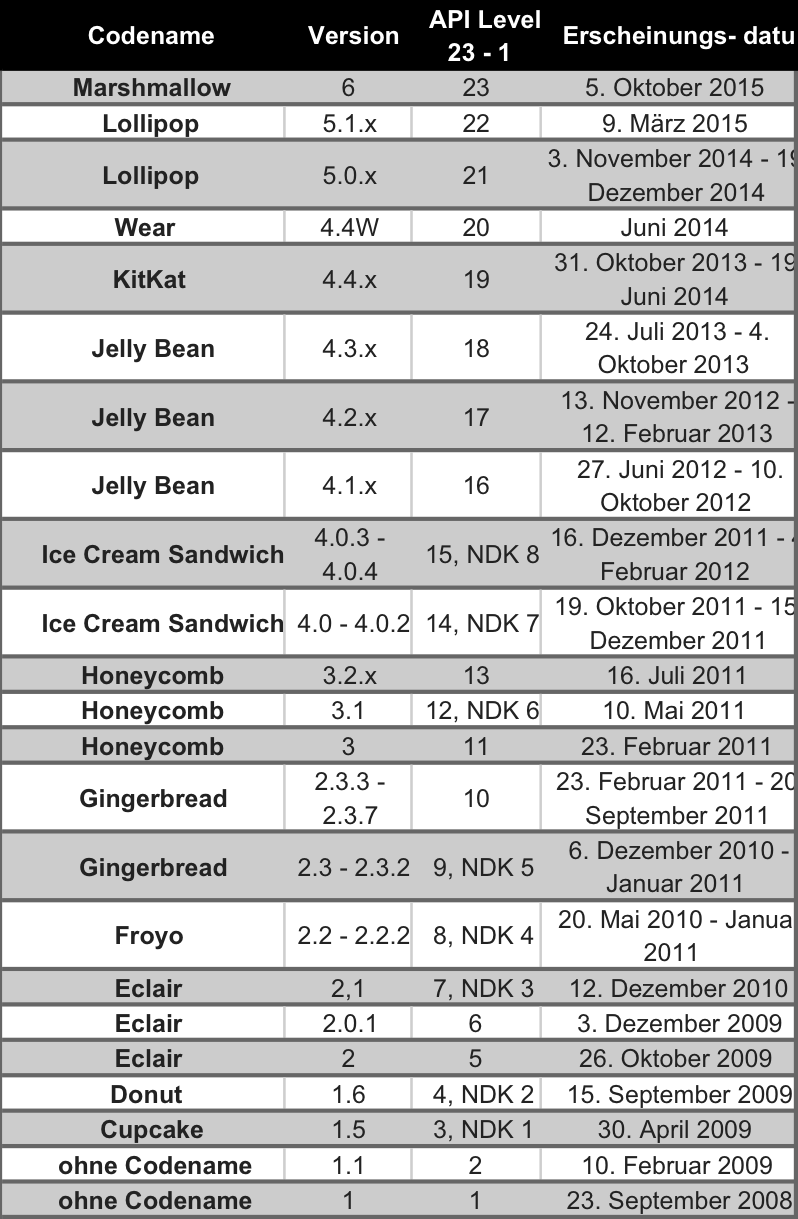
\includegraphics[width=0.5\textwidth]{Tabellen/Android_Versionen}
\caption{Android Versionen und ihr Erscheinungsdatum}\label{tab_android_vers}\citep{android_codenames,android_version_releases}
\end{table}

\clearpage

\subsection{Windows Phone Versionen}
%TODO

\section{Programmiersprachen}
In der nativen Entwicklung werden für jede Zielplattform bestimmte Programmiersprachen unterstützt. 

\subsection{iOS}
%TODO
\subsection{Android}
Android Applikationen werden in Java entwickelt. Demnach ist es notwendig vorab eine aktuelle Java Version (JDK) zu installieren. Diese wird von dem Unternehmen Oracle, mit der aktuellen Version 8 Update 66, vertrieben.
\citep{java_jdk}

\subsection{Windows Phone}
%TODO

%OPTIONAL!!!
%\subsection{Popularität der Programmiersprachen}

\section{Entwicklungsumgebungen}
Für die Entwicklung werden jeweilig verschiedene IDEs (Integrated Development Environment) seitens der Betreiber unterstützt und empfohlen. Eine Besonderheit bei IDEs für mobile Systeme ist die Unterstützung eines Simulators. Dieser simuliert ein spezifiziertes Gerät auf virtuelle Weise, um Entwicklungen direkt testen zu können.

\subsection{iOS}
%TODO
\subsection{Android}
Android empfiehlt das eigene Android Studio, welches die offizielle IDE für Android Entwicklung darstellt und zusätzlich das aktuelle SDK mitliefert. Android Studio basiert auf der IDE IntelliJ IDEA und ist frei verfügbar.\citep{android_studio} Alternativer Vorgänger ist die quelloffene IDE Eclipse.


\subsection{Windows Phone}
%TODO

%OPTIONAL!!!
%\section{Kompilierung}

%OPTIONAL!!!
%TODO: Kapitel 8
%\chapter{Stores für mobile Spiele}
%\section{Allgemeine Bedingungen für Entwickler}
%\section{Maximale App-Größe}
%\section{Anforderungen an den Quellcode}
%\section{Kosten und Abgaben}

%TODO: Kapitel 4
\chapter{Cross-Platform Entwicklung}
\section{Ziel}
\section{Funktionsweise}
\subsection{Technik}
\subsection{Geteilter Content}
\subsection{Übersetzung in die jeweiligen System}

%TODO: Kapitel 5
\chapter{Cross-Platform Frameworks}
\section{Tools und Anbieter zur Entwicklung}
\section{Verweis auf Bachelorarbeit: „Plattformabhängige und –unabhängige Entwicklung mobiler Anwendungen am Beispiel von Geo-Wikipedia-App“}
\section{Gamespezifische Frameworks und Engines}
\subsection{Monogame}
\subsection{Cocos2D}
\subsection{Libgdx}
\subsection{Unity}
\subsection{Unreal Engine}
\subsection{Weitere Frameworks}
\section{Entwicklungsumgebungen}
\subsection{Unterstützte IDEs}
\subsection{Systembedingte Einschränkungen}

%TODO: Kapitel 6
\chapter{Gegenüberstellung der Frameworks}
%Features und Einschränkungen
\section{Zielplattformen}
%\section{Skalierbarkeit der Menge der Plattformen} % ???
\section{Programmiersprachen}
\section{Unterstützung von 2D und 3D}
\section{Zugriff auf Hardware}%Accelerometer etc
\section{Free- und Pro- Versionen}
\section{Einfluss auf Einstellungen}
\section{Zusätzlich benötigte Software}
\section{Aktualität - Versionen - Community}
\section{Zukunftsaussichten}

%OPTIONAL!!!
%TODO: Kapitel 7
\chapter{Analyse der Marktanteile}
\section{Menge an Firmen und Entwicklern}
\section{Menge an Games}

%TODO: Kapitel 9
\chapter{Kosten-Nutzen Vergleich}
%Vergleichstabelle zu den Variationen der Projektanforderungen im Zusammenhang mit den Möglichkeiten und Kosten der Frameworks

%OPTIONAL!!!
%TODO: Kapitel 10
%\chapter{Grundgerüst und Aufbau eines Cross-Plattform Projekts}
%\section{Geteilter Content}
%\section{Plattformabhängiger Content}
%\section{Grundaufbau bei Engines}
%\section{Grundaufbau bei Frameworks}

%OPTIONAL!!!
%TODO: Kapitel 11
%\chapter{Game-typische Design Patterns und Architekturen}
%\section{Architekturen}
%\section{Patterns}
%\section{Verweis auf Bachelorarbeit: „Use of Design Patterns for mobile game Development“}

%OPTIONAL!!!
%TODO: Kapitel 12
%\chapter{Nutzen von Architekturen}
%\section{Pro}
%\subsection{Skalierbarkeit}
%\subsection{Lesbarkeit}
%\subsection{Wiederverwertbarkeit}
%\section{Contra}
%\subsection{KISS - Keep it simple stupid}

%TODO: Kapitel 13
\chapter{Konzeption einer Applikation}
\section{Ideen}
\section{Anforderungen}
\section{User Stories}

%TODO: Kapitel 14
\chapter{Implementierung der Applikation}
\section{Verwendete Frameworks und Engines}
\section{Verwendete APIs und SDKs}
\section{Assets und deren Verwendung}

\chapter{Analyse messbarer Metriken}
%Kosten, Performance, Akkuverbrauch, App-Daten-Aufteilung, Größe des benötigten Speichers, Größe des geteilten Contents, Stabilität, RAM, Code-Zeilen/-Größe, Entwicklungszeit(bedingt zu berücksichtigen)

\chapter{Vergleich der Messprotokolle}

\chapter{Fazit}



%--------------------- VERZEICHNISSE -------------------------------------

\listoffigures % Abbildungsverzeichnis erzeugen
\listoftables % Tabellenverzeichnis erzeugen

%------------------------------ LITERATURVERZEICHNIS----------------------
%TODO:Alphabetisch sortieren!
\begin{thebibliography}{}

\bibitem[Open Handset Alliance - Android Overview(2015)]{android_overview}
\emph{Overview of Android by the Open Handset Alliance},
\url{http://www.openhandsetalliance.com/android_overview.html}, letzter Zugriff: 24.11.2015

\bibitem[Open Handset Alliance - Alliance Overview(2015)]{alliance_overview}
\emph{Overview of the Open Handset Alliance},
\url{http://www.openhandsetalliance.com/oha_overview.html}, letzter Zugriff: 24.11.2015

\bibitem[Open Handset Alliance - Alliance Members(2015)]{alliance_members}
\emph{Members of the Open Handset Alliance},
\url{http://www.openhandsetalliance.com/oha_members.html}, letzter Zugriff: 24.11.2015

\bibitem[Android Source - Codenames, Tags, and Build Numbers(2015)]{android_codenames}
\emph{Codenames, Tags, and Build Numbers in the history of Android},
\url{https://source.android.com/source/build-numbers.html}, etzter Zugriff: 24.11.2015

\bibitem[Wikipedia - Liste von Android-Versionen(2015)]{android_version_releases}
\emph{Übersicht von allen Android Versionen mit Veröffentlichungsdatum},
\url{https://de.wikipedia.org/wiki/Liste_von_Android-Versionen}, letzter Zugriff: 24.11.2015

\bibitem[John Daintith(2004)]{native_software}
\emph{A Dictionary of Computing - native software},
\url{http://www.encyclopedia.com/doc/1O11-nativesoftware.html}, letzter Zugriff: 24.11.2015

\bibitem[Sue Smith(2013)]{android_sdk_requirements}
\emph{Android SDK Requirements},
\url{http://code.tutsplus.com/tutorials/android-sdk-requirements--mobile-20086}, letzter Zugriff: 24.11.2015

\bibitem[the iphone wiki(2015)]{ios_codenames}
\emph{Firmware},
\url{https://www.theiphonewiki.com/wiki/Firmware}, letzter Zugriff: 24.11.2015

\bibitem[Oracle - Java SE(2015)]{java_jdk}
\emph{Java SE Development Kit 8 Downloads},
\url{http://www.oracle.com/technetwork/java/javase/downloads/jdk8-downloads-2133151.html}, letzter Zugriff: 24.11.2015

\bibitem[Android Develop Tools(2015)]{android_studio}
\emph{Android Studio Overview},
\url{http://developer.android.com/tools/studio/index.html}, letzter Zugriff: 24.11.2015
%Quelle: http://developer.android.com/tools/studio/index.html

\end{thebibliography}
%----------------------------- EIGENSTÄNDIGKEITSERKLÄRUNG-----------------
\clearpage\thispagestyle{empty}
\eigen  % im header definiert
%----------------------------- ENDE --------------------------------------
\end{document}